\fancyhead[LE]{\fontsize{8.5pt}{10pt}\selectfont\textbf{\textsf{\thepage}}\quad \textbf{\textsf{CHƯƠNG 1}}\quad \textsf{Các hàm số và Mô hình}}
\fancyhead[RO]{\fontsize{8.5pt}{10pt}\selectfont\textsf{MỤC 1.1}\quad \textbf{\textsf{\thepage}}}

\noindent
\begin{minipage}[t]{0.265\textwidth}
    \fontsize{8pt}{10pt}\selectfont
    \vspace*{110pt}
    Các Trang Tra cứu nằm ở phần đầu và phần cuối của cuốn sách.

    \vspace{45pt}
    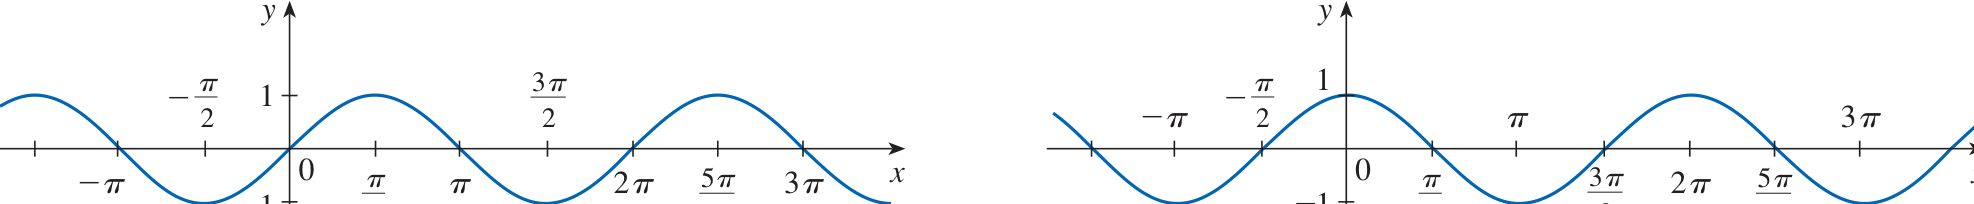
\includegraphics[width=0.92\linewidth]{images/p0065_fig19.png}
    \par\vspace{4pt}
    \textbf{\textsf{HÌNH 19}}
\end{minipage}%
\hfill
\begin{minipage}[t]{0.708\textwidth}
    \fontsize{9.3pt}{13.2pt}\selectfont
    Một ví dụ về hàm đại số xuất hiện trong thuyết tương đối. Khối lượng của một hạt có vận tốc $v$ là
    \begin{equation*}
    m = f(v) = \frac{m_0}{\sqrt{1 - v^2/c^2}}
    \end{equation*}
    trong đó $m_0$ là khối lượng nghỉ của hạt và $c = 3{,}0 \times 10^5\text{ km/s}$ là tốc độ ánh sáng trong chân không.

    \vspace{4pt}
    Các hàm số không phải là hàm đại số được gọi là các hàm \textbf{siêu việt}; chúng bao gồm các hàm lượng giác, hàm mũ và hàm logarit.

    \vspace{10pt}
    \noindent{\color{stewartcyan}\rule{1.2ex}{1.2ex}}\hspace{0.5em}\textbf{\textsf{\large Các hàm lượng giác}}\par\vspace{6pt}
    Lượng giác và các hàm lượng giác được ôn tập tại Trang Tra cứu 2 và trong Phụ lục D. Trong giải tích, quy ước là \emph{đơn vị radian} luôn luôn được sử dụng (trừ khi có chỉ định khác). Ví dụ, khi chúng ta sử dụng hàm số $f(x) = \sin x$, ta hiểu rằng $\sin x$ là sin của góc có số đo radian bằng $x$. Do đó, đồ thị của các hàm sin và cosin được cho như trong Hình 19.

    \vspace{65pt}
    Lưu ý rằng đối với cả hai hàm sin và cosin, tập xác định là $(-\infty, \infty)$ và tập giá trị là đoạn $[-1, 1]$. Do đó, với mọi giá trị của $x$, ta có
    \begin{center}
    \setlength{\fboxrule}{0.8pt}
    \setlength{\fboxsep}{7pt}
    \fcolorbox{stewartred}{white}{%
        \parbox{0.75\linewidth}{%
            \centering
            $-1 \leqslant \sin x \leqslant 1 \qquad\quad -1 \leqslant \cos x \leqslant 1$%
        }%
    }
    \end{center}
    hoặc theo ngôn ngữ giá trị tuyệt đối,
    \begin{equation*}
    |\sin x| \leqslant 1 \qquad |\cos x| \leqslant 1
    \end{equation*}

    Một tính chất quan trọng của các hàm sin và cosin là chúng là các hàm tuần hoàn và có chu kỳ $2\pi$. Điều này có nghĩa là, với mọi giá trị của $x$,
    \begin{center}
    \setlength{\fboxrule}{0.8pt}
    \setlength{\fboxsep}{7pt}
    \fcolorbox{stewartred}{white}{%
        \parbox{0.82\linewidth}{%
            \centering
            $\sin(x + 2\pi) = \sin x \qquad\quad \cos(x + 2\pi) = \cos x$%
        }%
    }
    \end{center}

    Bản chất tuần hoàn của các hàm số này khiến chúng rất thích hợp để mô hình hóa các hiện tượng lặp đi lặp lại như thủy triều, dao động lò xo và sóng âm. Chẳng hạn, trong Ví dụ 1.3.4 chúng ta sẽ thấy một mô hình hợp lý cho số giờ có ánh sáng ban ngày ở Philadelphia sau $t$ ngày kể từ ngày 1 tháng 1 được xác định bởi hàm số
    \begin{equation*}
    L(t) = 12 + 2{,}8 \sin\left[ \frac{2\pi}{365}(t - 80) \right]
    \end{equation*}
\end{minipage}